\documentclass{article}
\usepackage[hmargin=1in,vmargin=1.5in]{geometry}
\usepackage{amsmath}
\usepackage{amsfonts}
\usepackage{graphicx}
\usepackage{subcaption}
\usepackage{bm}
\newcommand{\A}{\bm A}
\newcommand{\x}{\bm x}
\newcommand{\y}{\bm y}
\newcommand{\z}{\bm z}
\renewcommand{\a}{\bm a}
\renewcommand{\b}{\bm b}
\renewcommand{\c}{\bm c}
\renewcommand{\d}{\bm d}
\renewcommand{\v}{\bm v}
\newcommand{\p}{\bm p}
\newcommand{\q}{\bm q}
\newcommand{\1}{\bm 1}
\title{Homework 2}
\author{Xinyi Gu, Songchen Tan}
\date{\today}
\begin{document}
\maketitle
\section{}
When we convert the polyhedron in the geometric form $\A\x\ge\b$ to standard form $\A'\x'=\b',\x'\ge0$, we will add a new variable for each inequality, therefore the extreme point in the standard form is not related to the extreme point in the geometric form. For example, $1x_1+0x_2\ge0$ is a valid polyhedron in $\mathbb R^2$ with no extreme points, and its corresponding standard form $x_1^+-x_1^--x_3=0, \x'=(x_1^+,x_1^-,x_2^+,x_2^-,x_3)\ge0$ has an extreme point $(0, 0, 0, 0, 0)$, which does not correspond to an extreme point in the geometric form.

\section{}

Dual problem:

\begin{align*}
    \max \quad & 3p_2 + 6 p_3  \\
    \text{s.t.} \quad & p_1 \leq 0 \\
    & p_2 \geq 0\\
    & p_3 \quad \text{free}\\
    & 2p_1 + 3p_2 - p_3 \geq 1 \\
    & 3p_1 + p_2 - p_3 \leq -1 \\
    & -p_1 + 4p_2 + 2p_3 \leq 0 \\
    & p_1 - 2p_2 + p_3 = 0
\end{align*}



\section{}
We denote $z=(x',y')'$, $v=(c',d')'$ such that we can reformulate the problem into minimizing $v'z$ subject to $(A, B)z=b$, $(D, 0)z\le f$ and $(0, G)z\le g$.

The dual problem is therefore maximizing $p'b+q'f+r'g$ where $p\in\mathbb R^{p_1}, q\in\mathbb R^{p_2}, r\in\mathbb R^{p_3}$, subject to

$$
\begin{cases}
    q\le 0\\
    r\le 0\\
    p'A+q'D=c\\
    p'B+r'G=d
\end{cases}
$$

Using the given data, we obtained that the optimal solution $\approx -236.41$ for both the primal and dual problem. (See code \verb|3.jl|.)

\section{}
\subsection*{(a)}

We denote the polynomial coefficients $a_0, \cdots, a_d$, so that the minimization problem is defined as

$$
\min_{a_i, i = 0,\cdots, d}\max_{j=1,\cdots,N}|f(x_j) - (a_0+a_1x_j^1+\cdots+a_dx_j^d)|
$$

Given $a_i$, let $m>0$ be the maximum, then we can express the problem as a LO over variables $\{a_i|i=0,\cdots,d\} \cup \{m\}$ that minimizes $m$ subject to

$$
\begin{cases}
    m \ge 0\\
    m \ge + f(x_j) - (a_0 + a_1x_j^1+\cdots+a_dx_j^d) & \forall j=1, \cdots, N\\
    m \ge - f(x_j) + (a_0 + a_1x_j^1+\cdots+a_dx_j^d) & \forall j=1, \cdots, N\\
\end{cases}
$$

\subsection*{(b)}
Dual problem:

Two primal constraints in (a), set dual variables as $p^{+}_j$ and $p^{-}_j$.

\begin{align*}
    \max \quad & \sum^{N}_{j=1} f(x_j)(p^{+}_j - p^{-}_j) & \\
    \text{s.t.} \quad & \sum^{N}_{j=1}(p^{+}_j + p^{-}_j) = 1 \\
    & \sum^{N}_{j=1}x^{i}_j (p^{+}_j - p^{-}_j) = 0, & i = 0, 1, \cdots, d \\
    & p^{+}_j, p^{-}_j \geq 0, & j = 1, \cdots, N
\end{align*}

\subsection*{(c)}
complementary slackness conditions:

$$
\begin{cases}
    (m - f(x_j) + (a_0 + a_1x_j^1+\cdots+a_dx_j^d)) p^{+}_j = 0 & \forall j=1, \cdots, N\\
    (m + f(x_j) - (a_0 + a_1x_j^1+\cdots+a_dx_j^d)) p^{-}_j = 0 & \forall j=1, \cdots, N\\
\end{cases}
$$

When $p^{+}_j, p^{-}_j > 0$, $m = |f(x_j) - p(x_j)|$, get maximum approximation error when $x_j$. From (b), we know that there are d+2 constraints in dual problem, results at most d+2 positive valunes in the optimal basic solutionmeans, means at most d+2 $x_j$ points get the maximum approximation error. 

\subsection*{(d)}

The approximation Chebyshev polynomials and the approximation errors are shown below. See Fig. 1.

\begin{figure}[!ht]
    \centering
    \begin{subfigure}[b]{0.48\textwidth}
        \centering
        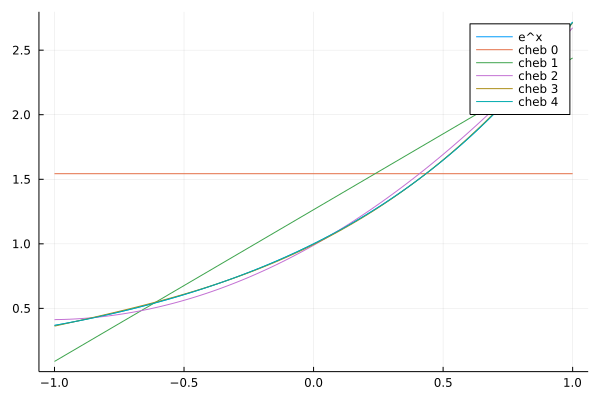
\includegraphics[width=\textwidth]{polynomial.png}
        \caption{Polynomials}
    \end{subfigure}
    \hfill
    \begin{subfigure}[b]{0.48\textwidth}
        \centering
        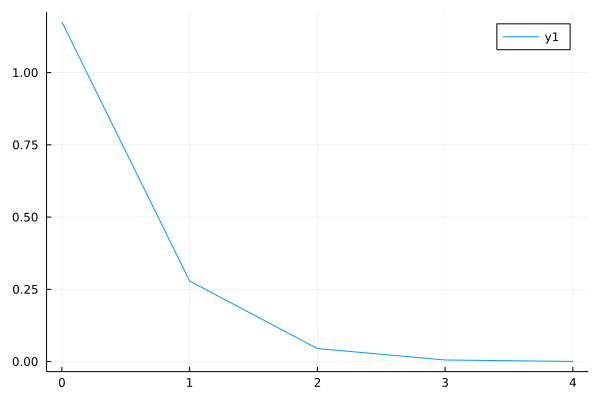
\includegraphics[width=\textwidth]{error.png}
        \caption{Errors}
    \end{subfigure}
       \caption{The Chebyshev polynomial and error for $d=0,1,2,3,4$}
\end{figure}

\subsection*{(e)}

We notice that the Chebyshev polynomials are visually closer to the original function $e^x$ in the given interval $[-1, 1]$. This is because Chebyshev polynomials consider all points in the interval and Taylor polynomials only consider the function value and derivatives at 0. See Fig. 2 in P4.

\begin{figure}[!ht]
    \centering
    \begin{subfigure}[b]{0.48\textwidth}
        \centering
        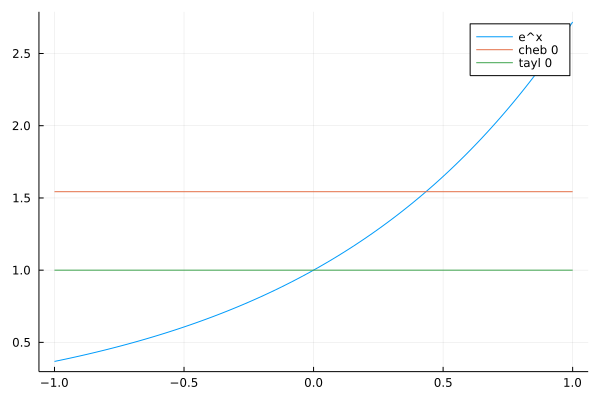
\includegraphics[width=\textwidth]{compare-0.png}
        \caption{$\deg p=0$}
    \end{subfigure}
    \hfill
    \begin{subfigure}[b]{0.48\textwidth}
        \centering
        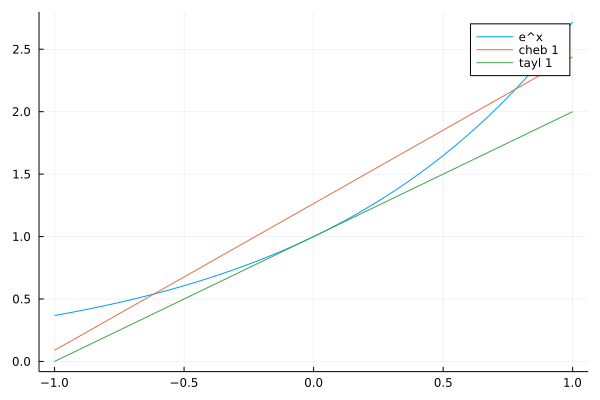
\includegraphics[width=\textwidth]{compare-1.png}
        \caption{$\deg p=1$}
    \end{subfigure}
    \newline
    \begin{subfigure}[b]{0.48\textwidth}
        \centering
        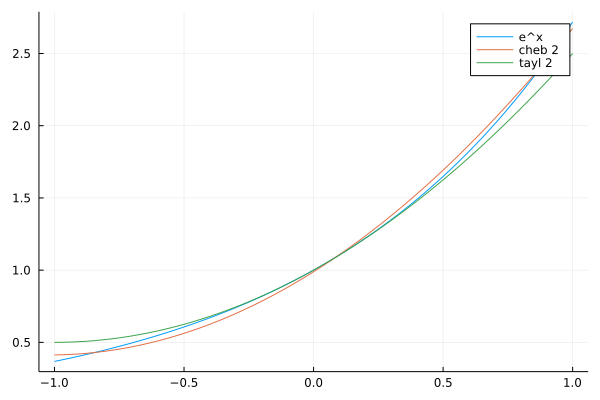
\includegraphics[width=\textwidth]{compare-2.png}
        \caption{$\deg p=2$}
    \end{subfigure}
    \hfill
    \begin{subfigure}[b]{0.48\textwidth}
        \centering
        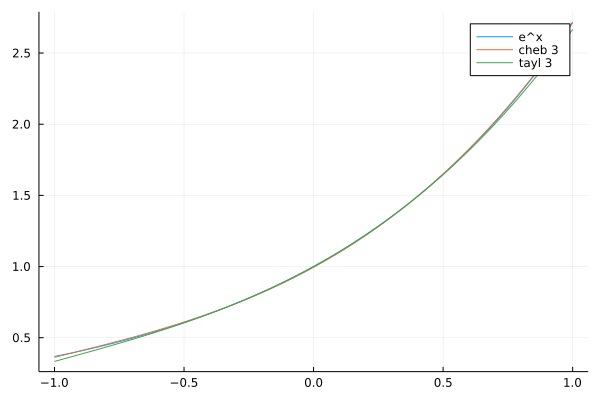
\includegraphics[width=\textwidth]{compare-3.png}
        \caption{$\deg p=3$}
    \end{subfigure}
    \newline
    \begin{subfigure}[b]{0.48\textwidth}
        \centering
        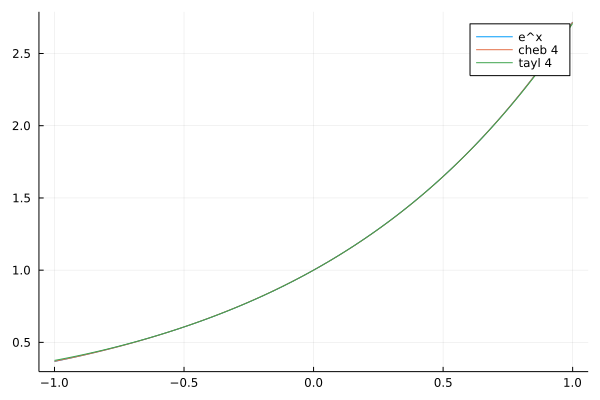
\includegraphics[width=\textwidth]{compare-4.png}
        \caption{$\deg p=4$}
    \end{subfigure}
    \caption{Comparison of Chebyshev polynomials and Taylor polynomials}
\end{figure}

\section{}

We start the proof by showing that (b) $\Rightarrow$ (a) is easy. If (b) holds, for all $\x>0$,

$$
\a^T\x=\sum_{j=1}^na_jx_j
\le\sum_{j=1}^n\sum_{i=1}^m\lambda_i(\a_{i})_j
=\sum_{i=1}^m\lambda_i(\a_i)^T\x\le\max_i(\a_i)^T\x
$$

Then we consider the LO problem: $\min z-\a^T\x$, subject to $(\a_i)^Tx-z\le 0$ ($i=1,\cdots,m$) and $x\ge0$. If (a) holds, then $z\ge\max_i(\a_i)^T\x\ge\a^Tx$, so the objective function is bounded. This problem is also feasible since $z$ is free. Now we denote $\y=-\x$ and define the resulting formulation as the primal problem: $\min \a^T\y+z$, subject to $(\a_i)^Ty+z\ge 0$ and $\y\le 0$. The dual of this problem would be $\max 0$, subject to

$$
\begin{cases}
(\lambda_1,\cdots,\lambda_m)\begin{pmatrix}
    \a_1^T\\\a_2^T\\\vdots\\\a_m^T
\end{pmatrix}
\ge\a^T\\
\sum_{i=1}^m\lambda_i=1\\
\lambda_i\ge0
\end{cases}
$$

According to the duality theorem, this problem is feasible, so (b) holds.

\end{document}
